% zhulong_arch_3.tex — TikZ redrawing of ZhuLong system architecture.
% Compiled standalone to figures/zhulong_arch_3.pdf (do NOT overwrite zhulong_arch_2.pdf).
% Content matches 3_design.tex caption/Description: four MCP tools + three platforms.
% Fonts: no extra font package (default CM); font size >= \scriptsize.
% Layout: 3 components in a row; four MCP tools in a 2x2 grid (compact, short) so the
% figure stays wide-and-short at width=\textwidth and does not push body to page 7.
\documentclass[border=2mm]{standalone}
\usepackage{tikz}
\usepackage{amssymb}
\usetikzlibrary{positioning,arrows.meta,shapes.geometric,fit,calc,backgrounds}
\begin{document}
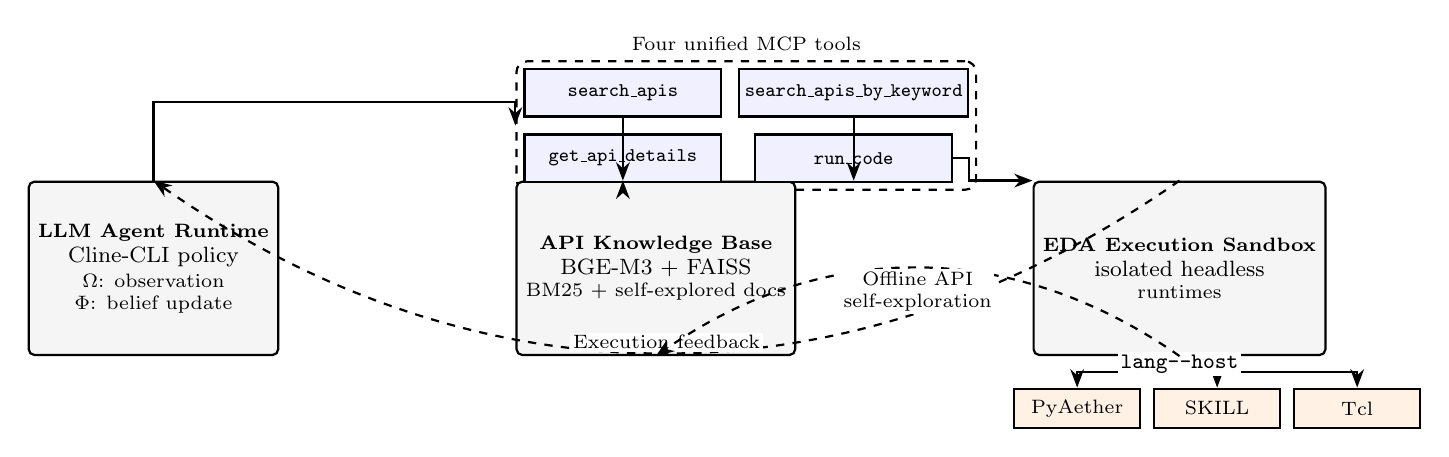
\begin{tikzpicture}[
  font=\scriptsize,
  >=Stealth,
  comp/.style={draw,thick,rounded corners=2pt,align=center,minimum height=22mm,minimum width=26mm,fill=gray!8},
  tool/.style={draw,thick,align=center,minimum width=25mm,minimum height=6mm,fill=blue!6,font=\scriptsize,inner sep=2pt},
  plat/.style={draw,thick,align=center,minimum width=16mm,minimum height=5mm,fill=orange!10,font=\scriptsize,inner sep=1.5pt},
  arr/.style={->,thick},
  arrd/.style={->,thick,dashed},
  lbl/.style={font=\scriptsize,fill=white,inner sep=1pt},
]

% ---- Three components in a row ----
\node[comp] (agent) at (0,0)
  {\textbf{LLM Agent Runtime}\\[1pt]
   \footnotesize Cline-CLI policy\\[1pt]
   $\Omega$: observation\\$\Phi$: belief update};
\node[comp,right=30mm of agent] (kb)
  {\textbf{API Knowledge Base}\\[1pt]
   \footnotesize BGE-M3 + FAISS\\ BM25 + self-explored docs};
\node[comp,right=30mm of kb] (sb)
  {\textbf{EDA Execution Sandbox}\\[1pt]
   \footnotesize isolated headless\\ runtimes};

% ---- Four MCP tools in a 2x2 grid above the KB ----
\node[tool,above=8mm of kb.north west,anchor=south west,xshift=1mm] (t1) {\texttt{search\_apis}};
\node[tool,right=2mm of t1] (t2) {\texttt{search\_apis\_by\_keyword}};
\node[tool,below=2mm of t1] (t3) {\texttt{get\_api\_details}};
\node[tool,below=2mm of t2] (t4) {\texttt{run\_code}};

\begin{scope}[on background layer]
  \node[draw,thick,dashed,rounded corners,fit=(t1)(t2)(t3)(t4),
        inner sep=2.5pt,label={[font=\scriptsize]above:Four unified MCP tools}] (mcp) {};
\end{scope}

% ---- Three platforms / languages under the sandbox ----
\node[plat,below=4mm of sb.south,anchor=north,xshift=-13mm] (p1) {PyAether};
\node[plat,right=1.5mm of p1] (p2) {SKILL};
\node[plat,right=1.5mm of p2] (p3) {Tcl};

% ---- Agent -> MCP tools (one arrow to the group) ----
\draw[arr] (agent.north) -- ++(0,10mm) -| (mcp.west);

% ---- MCP tools -> KB (search/get, left column + top-right) ----
\draw[arr] (t3.south) -- (kb.north -| t3.south);
\draw[arr] (t1.south) -- (t1.south |- kb.north);
\draw[arr] (t2.south) -- (t2.south |- kb.north);

% ---- run_code -> Sandbox ----
\draw[arr] (t4.east) -- ++(2mm,0) |- (sb.north west);

% ---- lang-host dispatch to platforms ----
\draw[arr] (sb.south) -- ++(0,-2mm) -| (p1.north);
\draw[arr] (sb.south) -- ++(0,-2mm) -| (p2.north);
\draw[arr] (sb.south) -- ++(0,-2mm) -| (p3.north);
\node[lbl] at ([yshift=-1mm]sb.south) {\footnotesize \texttt{lang--host}};

% ---- Execution feedback loop: sandbox -> agent (curved back, top) ----
\draw[arrd] (sb.north) to[bend left=35] node[lbl,above]{Execution feedback} (agent.north);

% ---- Offline API self-exploration: sandbox -> KB (dashed back-edge, bottom) ----
\draw[arrd] (sb.south) to[bend right=35] node[lbl,below,align=center]{Offline API\\self-exploration} (kb.south);

\end{tikzpicture}
\end{document}
